From the above section, it is easy to see that, with different CPU frequency, both stretched replication and shadow replication can have differernt response time, task reliability, and energy consumption. In order to derive the frequency for stretched replicaiton and shadow replication respectively, we come up with the following problem: Given a task and its task reliability target, determine the frequency assignment such that the energy consumption is minimized while guarantee that the task can be completed before its deadline with required reliability. 

\subsection{Problem formulation}
Assuming CPU frequency is continuous, the problem can be mathematically formulated as:

\begin{align}
\min_{\sigma}\quad\quad    & E \\
s.t.              \quad\quad                   & \sigma_{min} \leq \sigma \leq \sigma_{max} \\
                                     & T \leq P \\
                                     & R_{target} \leq R 
\end{align} 

%\begin{equation}
%\label{optimization_problem}
%%\setlength{\abovedisplayskip}{14pt}
%\begin{alignedat}{2}
%\min_{\sigma}    & E \\
%s.t.                                 & \sigma_{min} \leq \sigma \leq \sigma_{max} \\
%                                     & T \leq P \\
%                                     & R_{target} \leq R 
%\end{alignedat}
%\end{equation}

Above, Equation (1) says the objective is to minimize energy consumption. Constraint (1) ensures a valid frequency is used for each task instance. For stretched replication, $\sigma_r$ need to satisfy this requirement, and for shadow replication, $\sigma_m$, $\sigma_b$, and $\sigma_a$ all need to satisfy this condition. Constraint (3) says the task'c completion time should be eariler than the deadline. For shadow replication, this is equivalent to that the shadow can complete before deadline. The last constraint requires that the task reliability is no lower than the specified requirement. 

This is a nonlinear optimization problem that can be solved by available tools like MatLab. 

\subsection{Analysis}
We programmed the energy-optimal replication problem with MatLab and used the nonlinear optimiation algorithms implemented in MatLab to solve the problem. However, this approach is quite time-consuming. It takes more than half an hour to solve one instance of the problem. Therefore, we decide to take another path that uses brute force search to find out the optimal frequency assignment. This approach ended up to be much faster than the first approach, as a processor should only have a few valid frequency choices. 

Below we show some results in Fig.~\ref{fig:failure_impact} and Fig.~\ref{fig:utilization_impact}.  

\begin{figure}[!t]
	\begin{center}
		\subfigure[Energy consumption]
		{
			\label{fig:en_failure_10_100}
			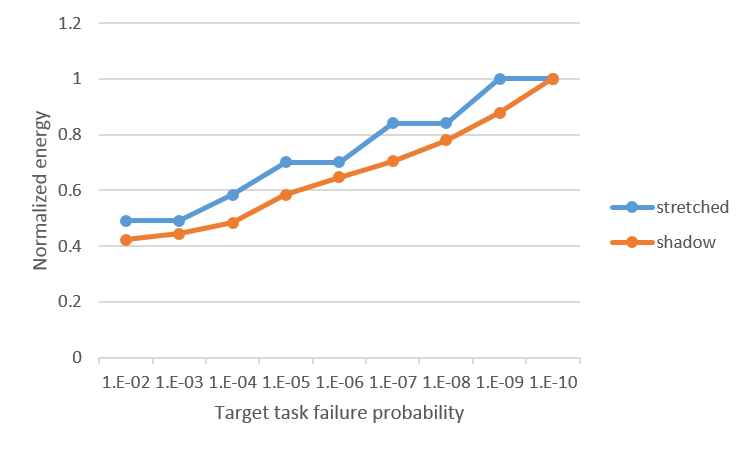
\includegraphics[width=0.45\columnwidth]{Figures/energy_vs_failure_10_100}
		} 
		\subfigure[CPU frequency]
		{
			\label{fig:speed_failure_10_100}
			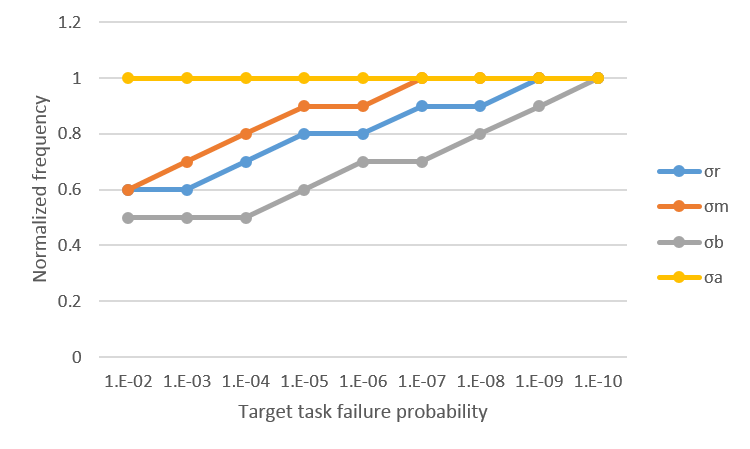
\includegraphics[width=0.45\columnwidth]{Figures/speed_vs_failure_10_100}
		} 
	\end{center}
	%\vskip -0.22in 
	\caption{Impact of target task failure probability on frequency assignment and energy consumption}
	\label{fig:failure_impact}
\end{figure}

\begin{figure}[!t]
	\begin{center}
		\subfigure[Energy consumption]
		{
			\label{fig:en_util_10}
			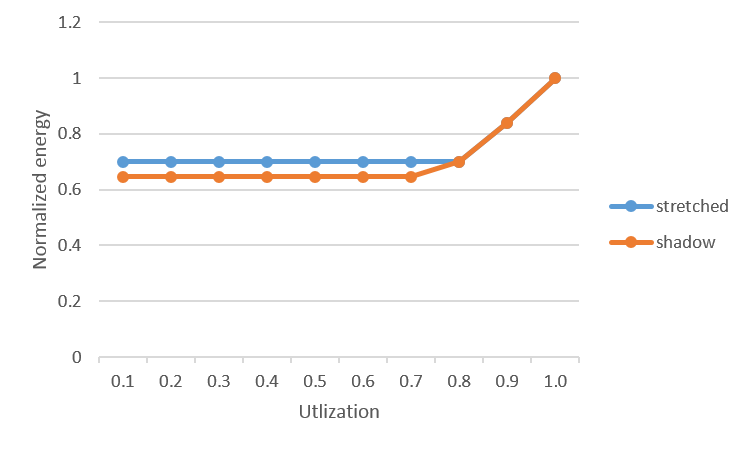
\includegraphics[width=0.45\columnwidth]{Figures/energy_vs_uti_10}
		} 
		\subfigure[CPU frequency]
		{
			\label{fig:speed_util_10}
			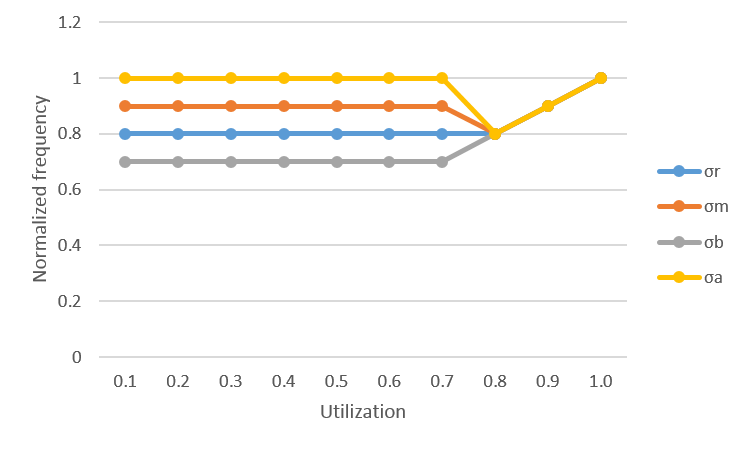
\includegraphics[width=0.45\columnwidth]{Figures/speed_vs_uti_10}
		} 
	\end{center}
	%\vskip -0.22in 
	\caption{Impact of utilization on frequency assignment and energy consumption}
	\label{fig:utilization_impact}
\end{figure}


